\section{Auswertung}
\label{sec:Auswertung}
\subsection{Messung der Topografie einer Mikrostruktur}
Im Verlauf der ersten Versuchsreihe werden verschiedene Strukturformen auf einer Mikrostrukturprobe betrachtet.
Mittels des AFM-Aufbaus werden von den drei vorhandenen Strukturen AFM-Bilder aufgenommen.
Es wird jeweils eine $(20 \times 20) \, \mu m$ gro{\ss}e Fl\"ache vermessen.
In den Abbildungen (\ref{abb:kreis}) bis (\ref{abb:streif}) sind diese Bilder zu sehen.
Abgebildet sind nicht nur die AFM-Aufnahmen, sondern auch die Strecken, welche vermessen wurden.
\begin{figure}[H]
\centering
	\begin{subfigure}[t]{0.45\textwidth}
	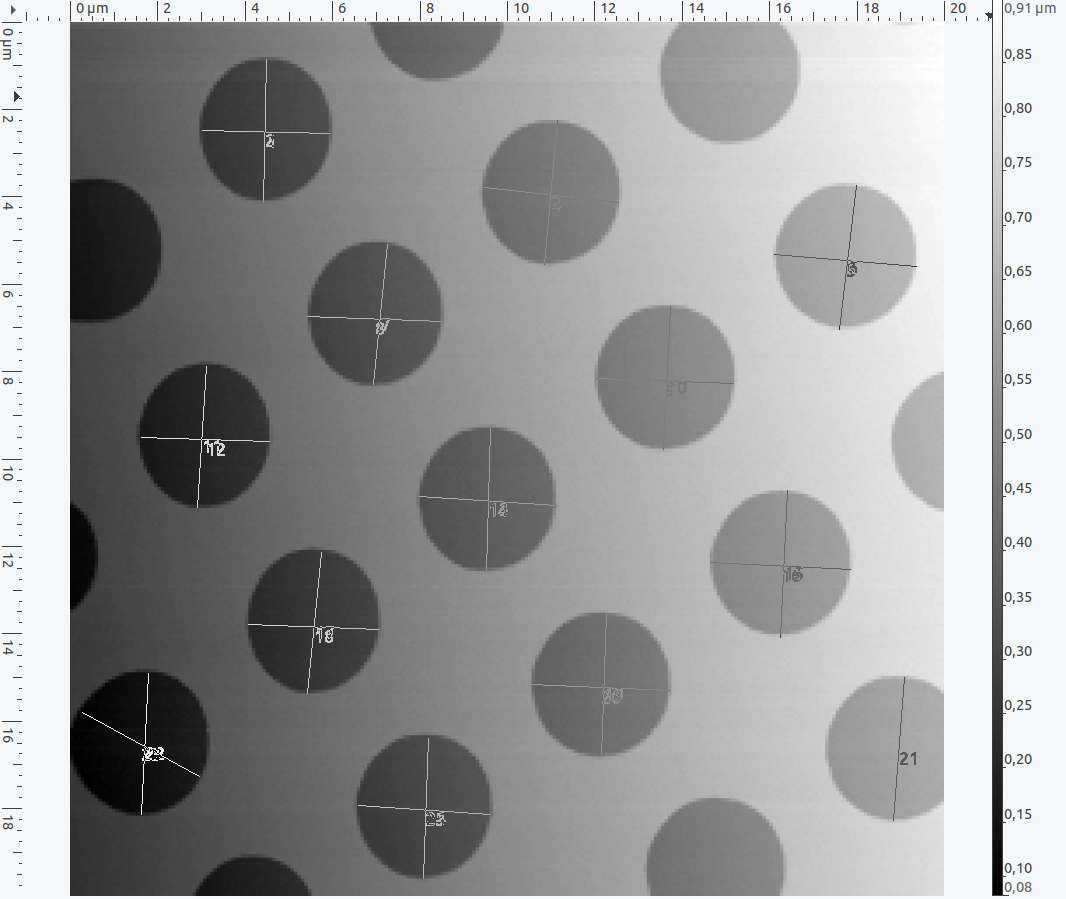
\includegraphics[width=\textwidth]{AFM_auswertung/Kreis_durch_vor.png}
	\caption{Vermessung des Kreisdurchmessers.}
	\label{abb:kreisa}
	\end{subfigure}
	~
	\begin{subfigure}[t]{0.45\textwidth}
	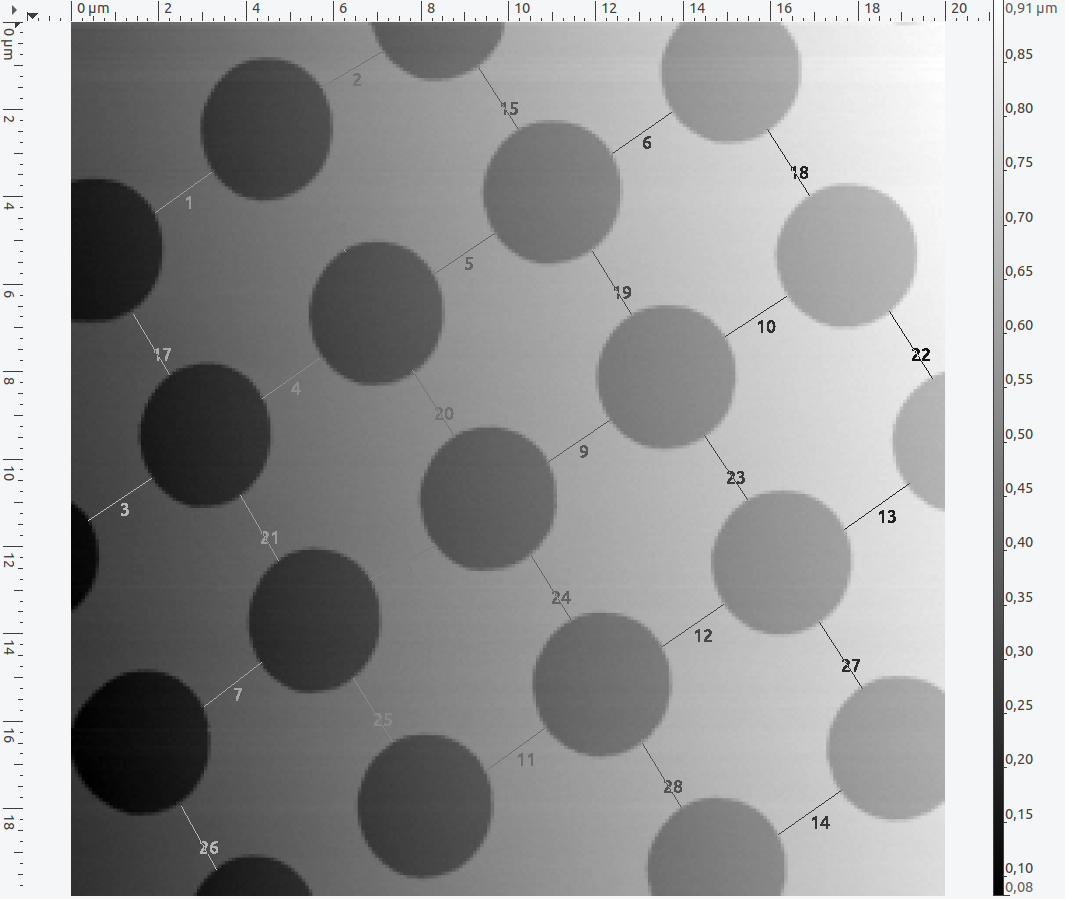
\includegraphics[width=\textwidth]{AFM_auswertung/Kreis_abs_vor.png}
	\caption{Bestimmung des Abstands zwischen den Kreisen.}
	\label{abb:kreisb}
	\end{subfigure}
\caption{Vermessung der Kreisstruktur auf der Mikrostrukturprobe. Aufgenommen wurde eine Fl\"ache der Gr\"o{\ss}e von $(20 \times 20) \, \mu m$. Zur Vermessung der jeweiligen Strecken wurde das 'distance and directinos-Tool' des Auswertungsprogramm Gwyddion verwendet.}
\label{abb:kreis}
\end{figure}
%
\begin{figure}[H]
\centering
	\begin{subfigure}[t]{0.45\textwidth}
	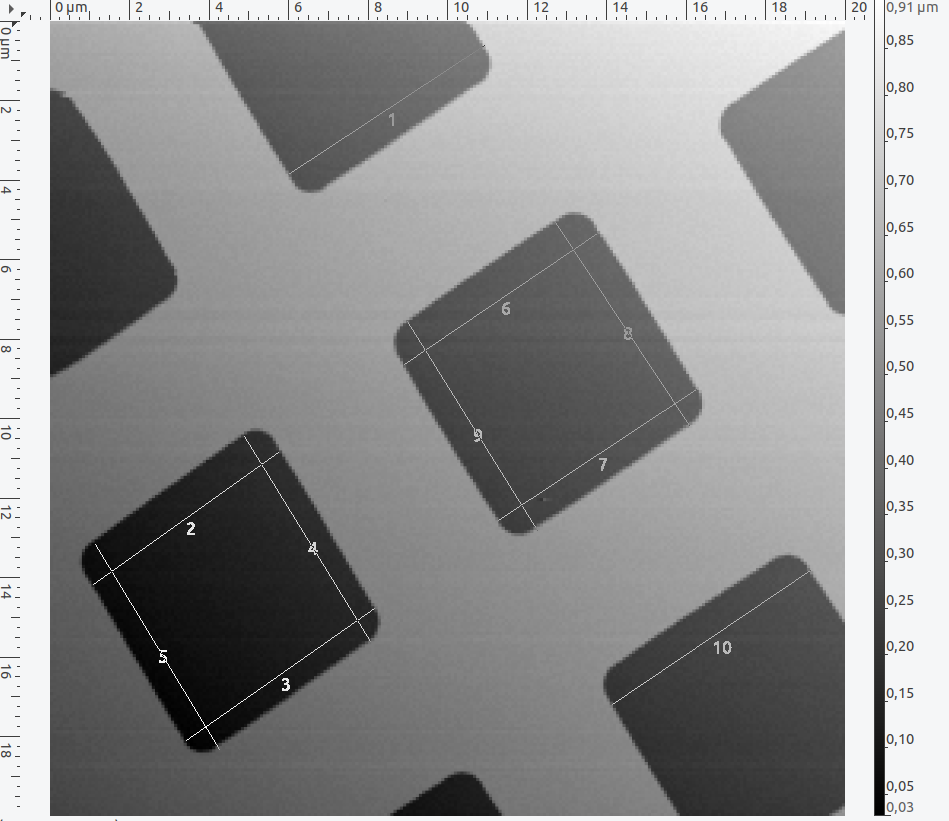
\includegraphics[width=\textwidth]{AFM_auswertung/quad_durch_vor.png}
	\caption{Vermessung der Quadratgr\"o{\ss}e.}
	\label{abb:quada}
	\end{subfigure}
	~
	\begin{subfigure}[t]{0.45\textwidth}
	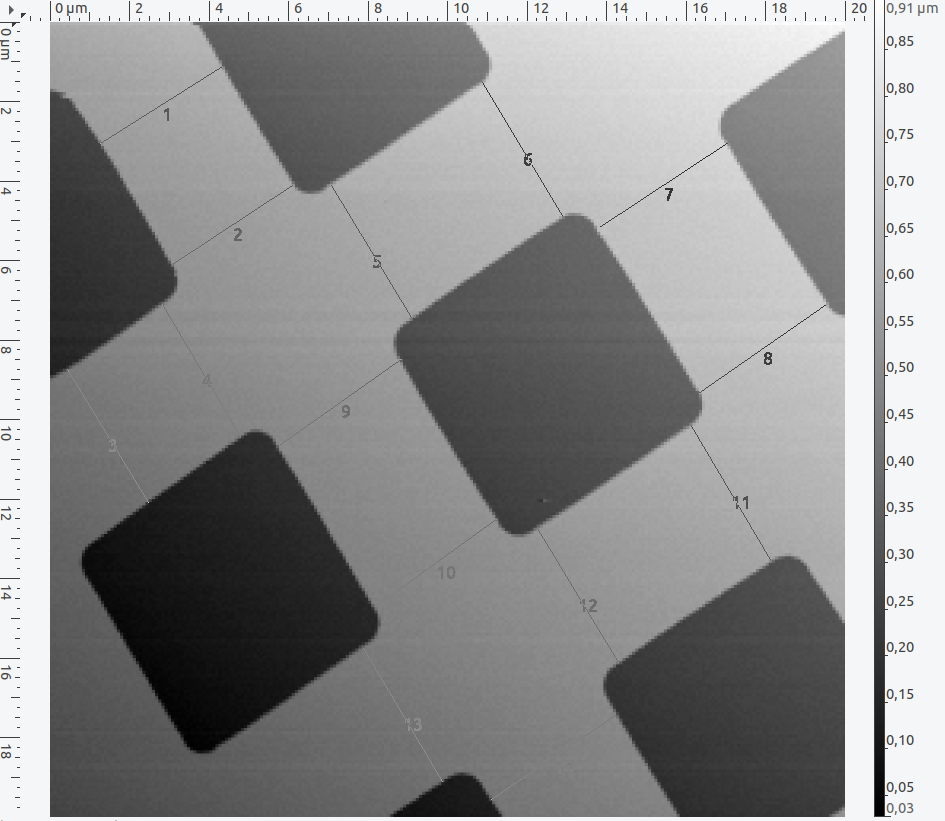
\includegraphics[width=\textwidth]{AFM_auswertung/quad_abb_vor.png}
	\caption{Bestimmung des Abstands zwischen den Quadraten.}
	\label{abb:quadb}
	\end{subfigure}
\caption{Vermessung der Quadratstruktur auf der Mikrostrukturprobe. Aufgenommen wurde eine Fl\"ache der Gr\"o{\ss}e von $(20 \times 20) \, \mu m$. Zur Vermessung der jeweiligen Strecken wurde das 'distance and directinos-Tool' des Auswertungsprogramm Gwyddion verwendet.}
\label{abb:quad}
\end{figure}
%
\begin{figure}[H]
\centering
	\begin{subfigure}[t]{0.45\textwidth}
	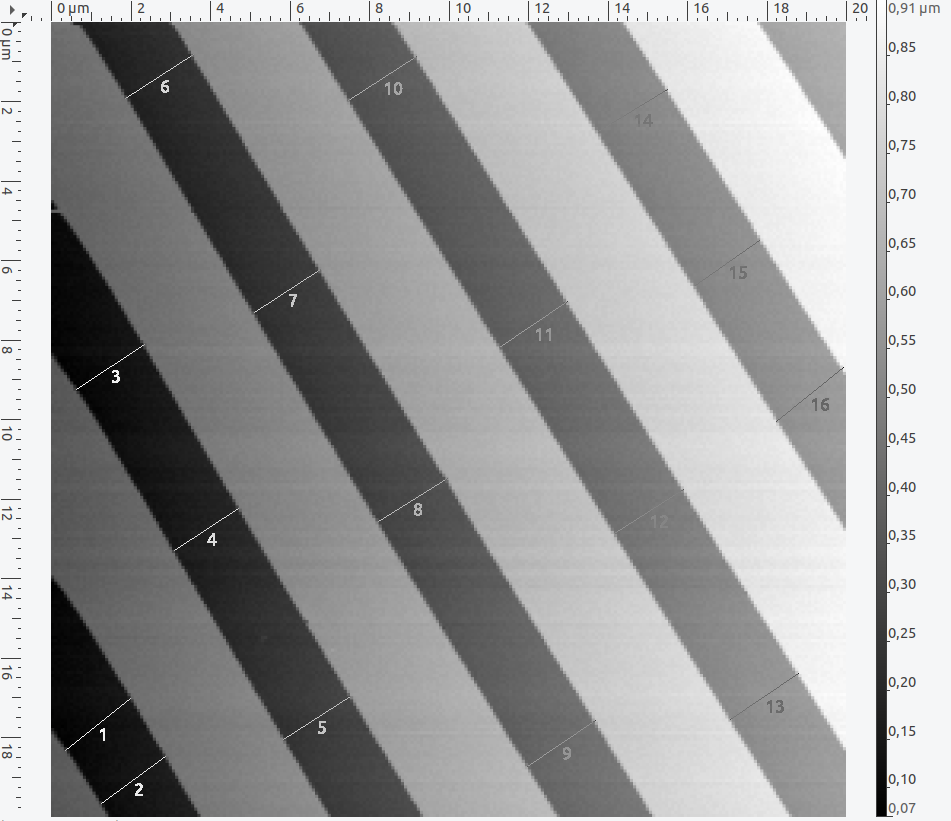
\includegraphics[width=\textwidth]{AFM_auswertung/streif_durch_vor.png}
	\caption{Vermessung der Streifenbreite.}
	\label{abb:streifa}
	\end{subfigure}
	~
	\begin{subfigure}[t]{0.45\textwidth}
	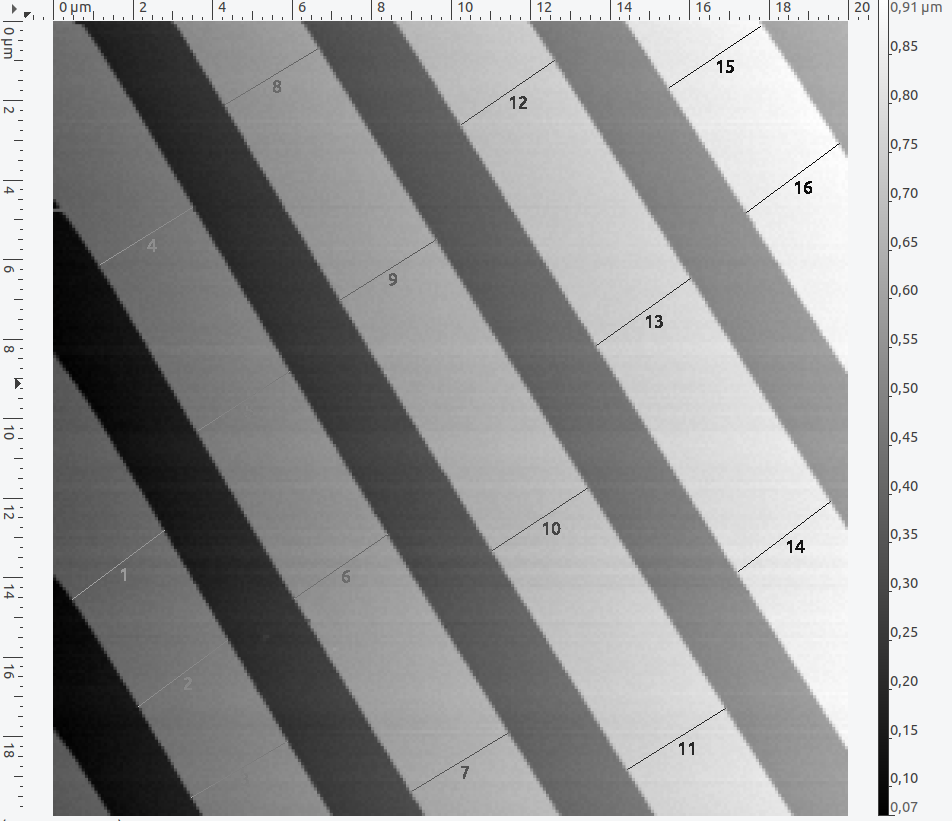
\includegraphics[width=\textwidth]{AFM_auswertung/streif_abb_vor.png}
	\caption{Vermessung des Abstands zwischen zwei Streifen.}
	\label{abb:streifb}
	\end{subfigure}
\caption{Vermessung der Streifen auf der Mikrostrukturprobe. Aufgenommen wurde eine Fl\"ache der Gr\"o{\ss}e von $(20 \times 20) \, \mu m$. Zur Vermessung der jeweiligen Strecken wurde das 'distance and directinos-Tool' des Auswertungsprogramm Gwyddion verwendet.}
\label{abb:streif}
\end{figure}
%
Diese sind in den einzelnen Bildern mit Nummern versehen und wurden mit Hilfe des Auswertungsprogramm Gwyddion erstellt.
In Tabelle (\ref{tab:auf1}) sind die Mittelwerte der aufgenommenen Werte aufgelistet.
Die experimentell bestimmten Daten werden mit den Strukturabst\"anden aus dem Datenblatt \cite{sample} verglichen.
Diese sind, genau wie die zugeh\"ohrigen Abweichungen, auch in Tabelle (\ref{tab:auf1}) festgehalten.
\begin{table}
	\centering
	\caption{Messwerte der Mikrostrukturprobe. Aufgelistet sind die gemittelten Werte der vermessenen Strecken und Abst\"ande. Der Strukturabstand ergibt sich aus der Summer von Gr\"o{\ss}e und Abstand der Mikrostruktur.}
\begin{tabular}{|r|ccc|}
	\hline
	{} & {Kreis} & {Quadrat} & {Streifen} \\
	\hline
	Größe / $\mu m$ & $3,177 \pm 0,096$ & $5,958 \pm 0,120$ & $2,037 \pm 0,039$ \\
	Abstand / $\mu m$ & $1,688 \pm 0,052$ & $3,839 \pm 0,089$ & $2,832 \pm 0,061$ \\
	Struckturabstand / $\mu m$ & $4,865 \pm 0,109$ & $ 9,797 \pm 0,149$ & $4,869 \pm 0,072$ \\
	Datenblatt / $\mu m$ & 5 & 10 & 5 \\
	Abweichung / \%	& 2,7 & 2,03 & 2,62 \\
	\hline
\end{tabular}
\label{tab:auf1}
\end{table}


\subsection{Topographie einer CD, DVD und Blu-ray}
Im zweiten Teil des Versuches wird die Oberfl\"ache von drei unterschiedliche Speichermedien, eine CD, eine DVD und eine Blu-ray, mit dem AFM untersucht.
Bevor die aufgenommenen Bilder und Daten mit Gwyddion ausgewertet werden, werden die Bilder gegl\"attet.
Hierf\"ur werden bearbeitungs Tool von Gwyddion verwendet, welche den Hintergrund entfernen und einzelne Zeilen mit verschiedenen Methoden ausrichten.
In Abbildung sind die bearbeiteten 3D-AFM-Bilder der drei unterschiedliche Speichermedien zu sehen.
\begin{figure}[H]
\centering
	\begin{subfigure}[t]{0.45\textwidth}
	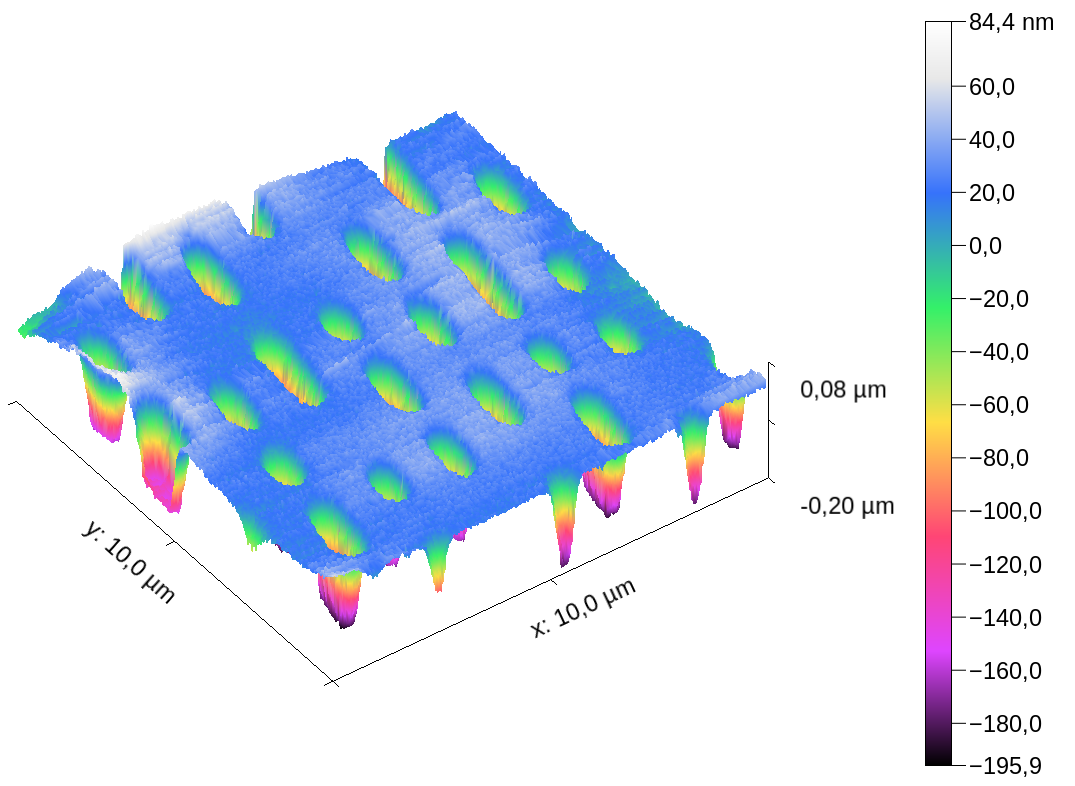
\includegraphics[width=\textwidth]{AFM_auswertung/cd_3D.png}
	\caption{3D-AFM-Bild einer CD Oberfl\"ache der Gr\"o{\ss}e $(10 \times 10) \, \mu m$.}
	\label{abb:cd_3d}
	\end{subfigure}
	~
	\begin{subfigure}[t]{0.45\textwidth}
	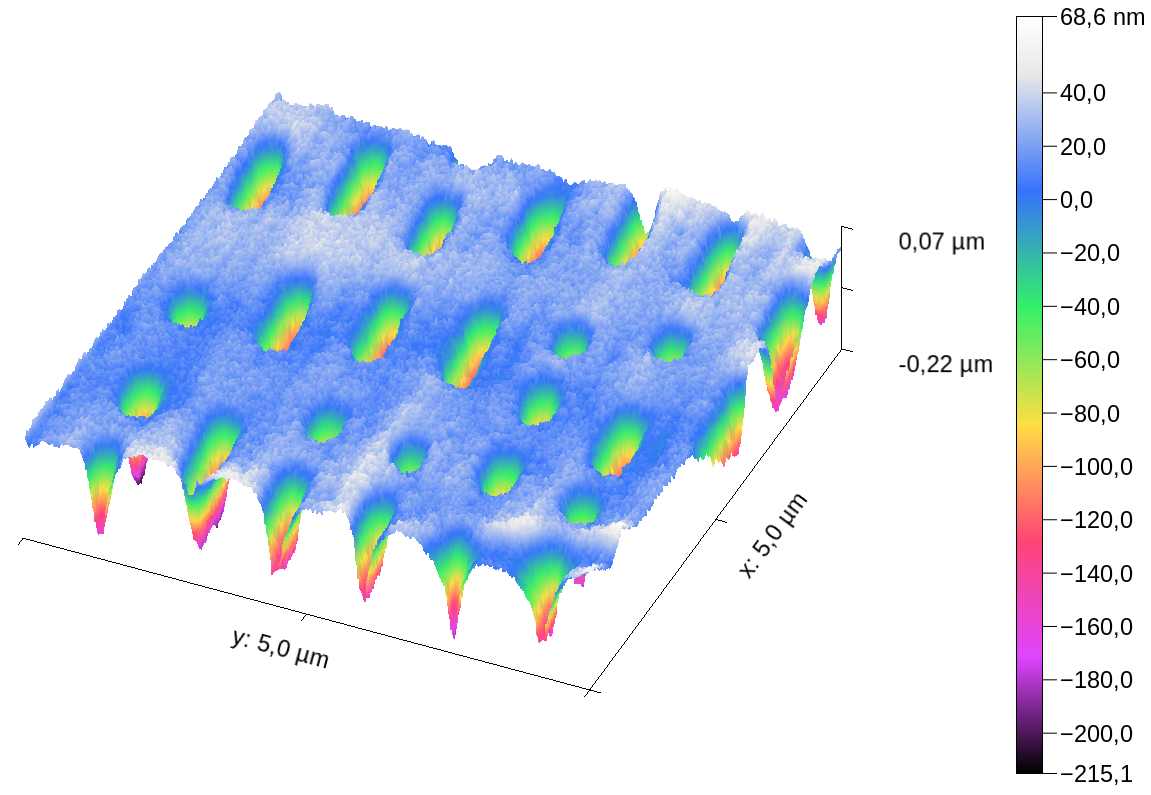
\includegraphics[width=\textwidth]{AFM_auswertung/dvd_3d.png}
	\caption{3D-AFM-Bild einer DVD Oberfl\"ache der Gr\"o{\ss}e $(5 \times 5) \, \mu m$.}
	\label{abb:dvd_3d}
	\end{subfigure}
	~
	\begin{subfigure}[t]{0.45\textwidth}
	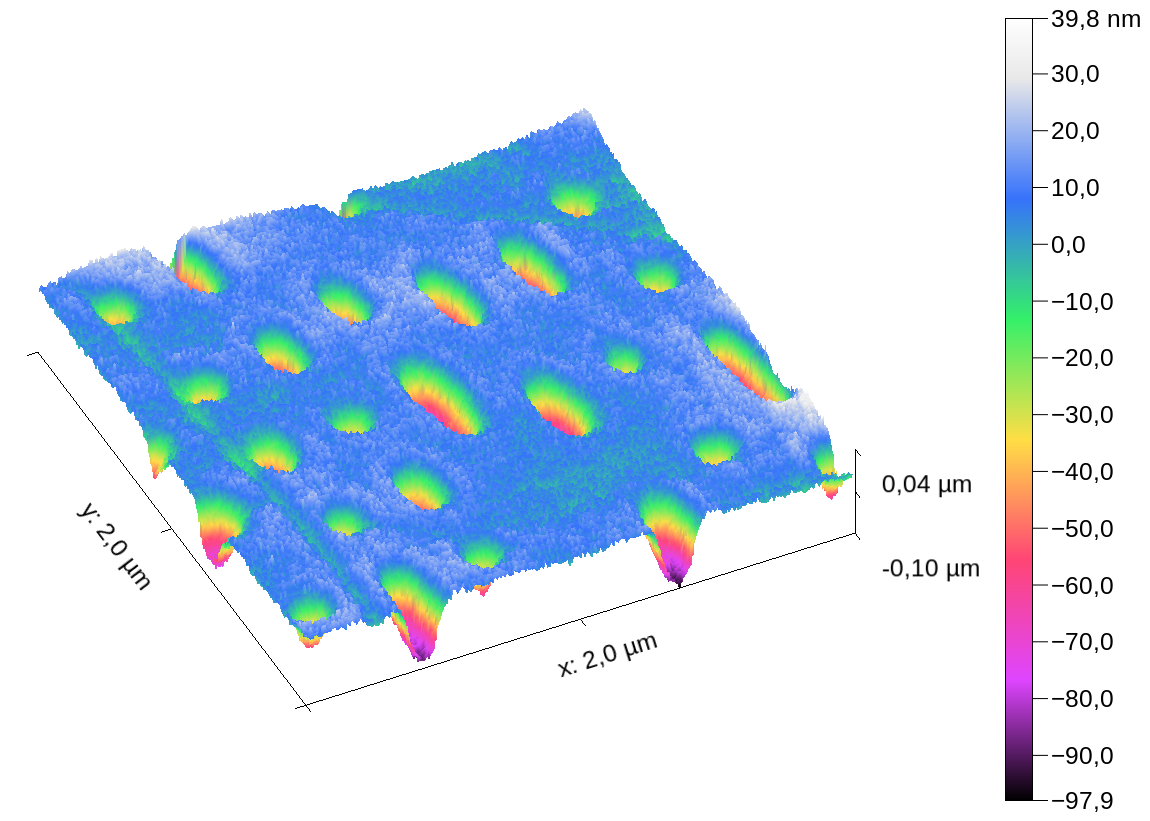
\includegraphics[width=\textwidth]{AFM_auswertung/bluray_3d.png}
	\caption{3D-AFM-Bild einer Blu-ray Oberfl\"ache der Gr\"o{\ss}e $(2 \times 2) \, \mu m$.}
	\label{abb:br_3d}
	\end{subfigure}
\caption{Dargestellt sind hier in 3D die bearbeiteten AFM-Aufnahmen der drei zu untersuchenden Speichermedien.}
\label{abb:3d}
\end{figure}
Um die Speicherkapazit\"at der einzelnen Medien absch\"atzen zu k\"onnen, werden Gr\"o{\ss}e und Abst\"ande der Pits gemessen.
Dzu werden Pitbreite, minimale und maximale L\"ange der Pits sowie der Abstand zwischen zwei Pitspuren mit Hilfe Gwyddion bestimmt.
In Abbildung (\ref{abb:CD}) sind beisielhaft f\"ur die CD die AFM-Bilde hierzu abgebildet.
Die entsprechenden Aufnahmen der DVD und Blu-ray sind im Anhang zu finden (Abbildungen (\ref{abb:DVD}) und (\ref{abb:BluRay})).
\begin{figure}[H]
\centering
	\begin{subfigure}[t]{0.4\textwidth}
	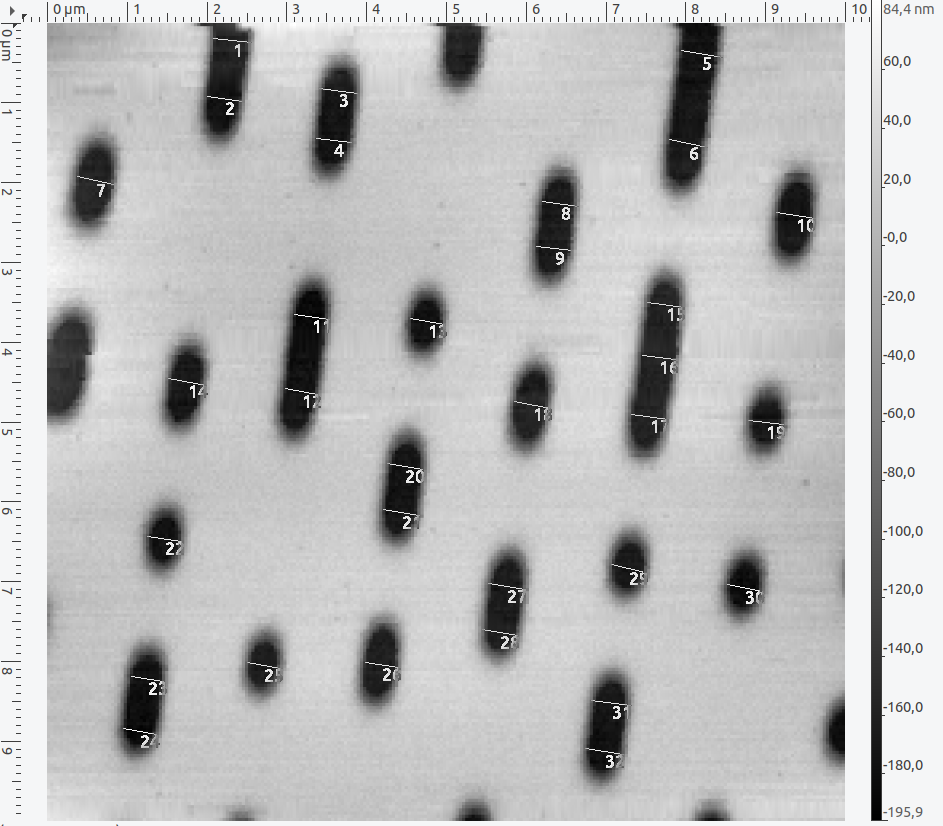
\includegraphics[width=\textwidth]{AFM_auswertung/cd_breite.png}
	\caption{.}
	\label{abb:}
	\end{subfigure}
	~
	\begin{subfigure}[t]{0.4\textwidth}
	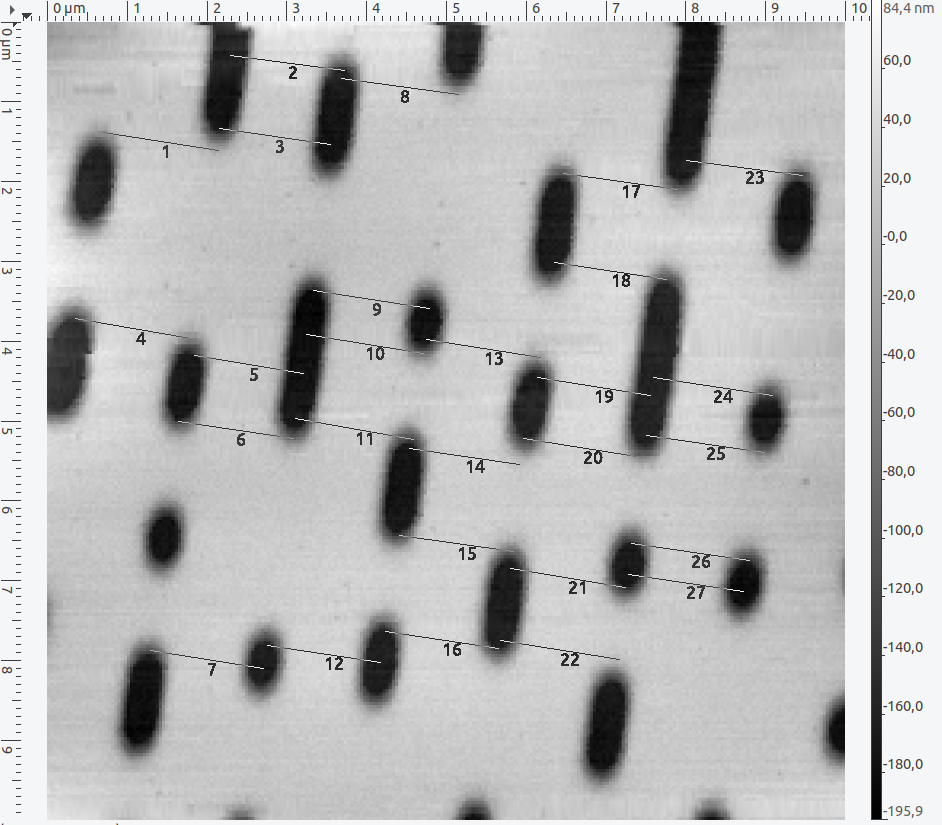
\includegraphics[width=\textwidth]{AFM_auswertung/cd_abstand.png}
	\caption{.}
	\label{abb:}
	\end{subfigure}
	\\
	\begin{subfigure}[t]{0.4\textwidth}
	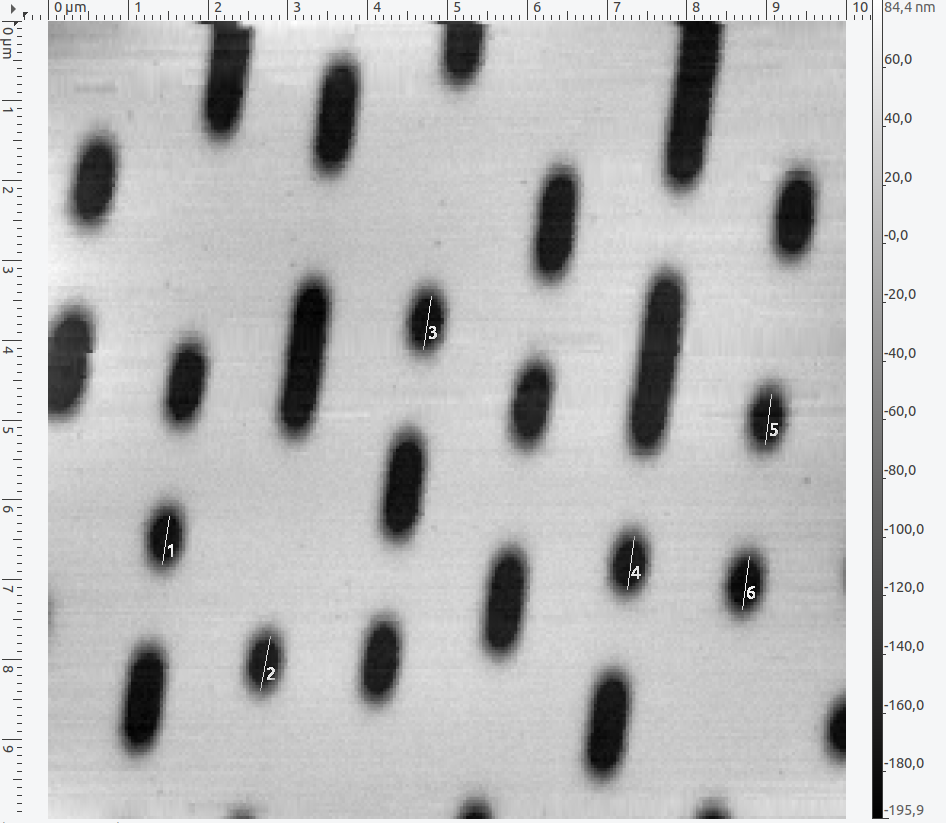
\includegraphics[width=\textwidth]{AFM_auswertung/cd_Lmin.png}
	\caption{.}
	\label{abb:}
	\end{subfigure}
	~
	\begin{subfigure}[t]{0.4\textwidth}
	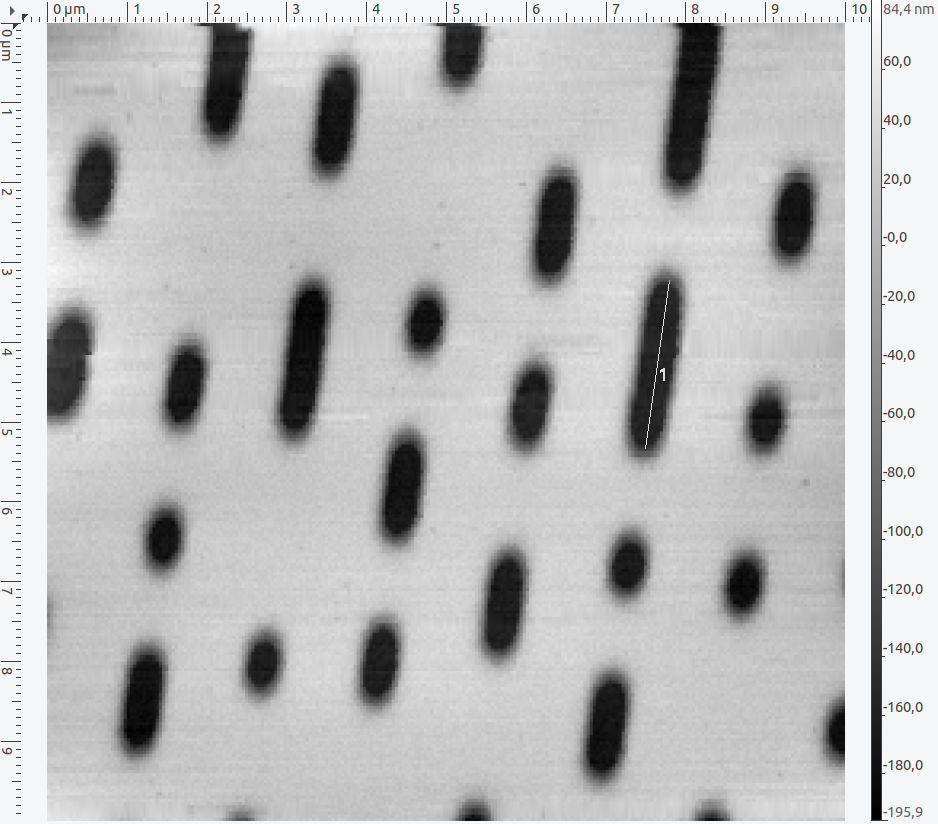
\includegraphics[width=\textwidth]{AFM_auswertung/cd_Lmax.png}
	\caption{.}
	\label{abb:}
	\end{subfigure}
\caption{Gezeigt ist hier .}
\label{abb:CD}
\end{figure}

\begin{figure}[H]
\centering
	\begin{subfigure}[t]{0.3\textwidth}
	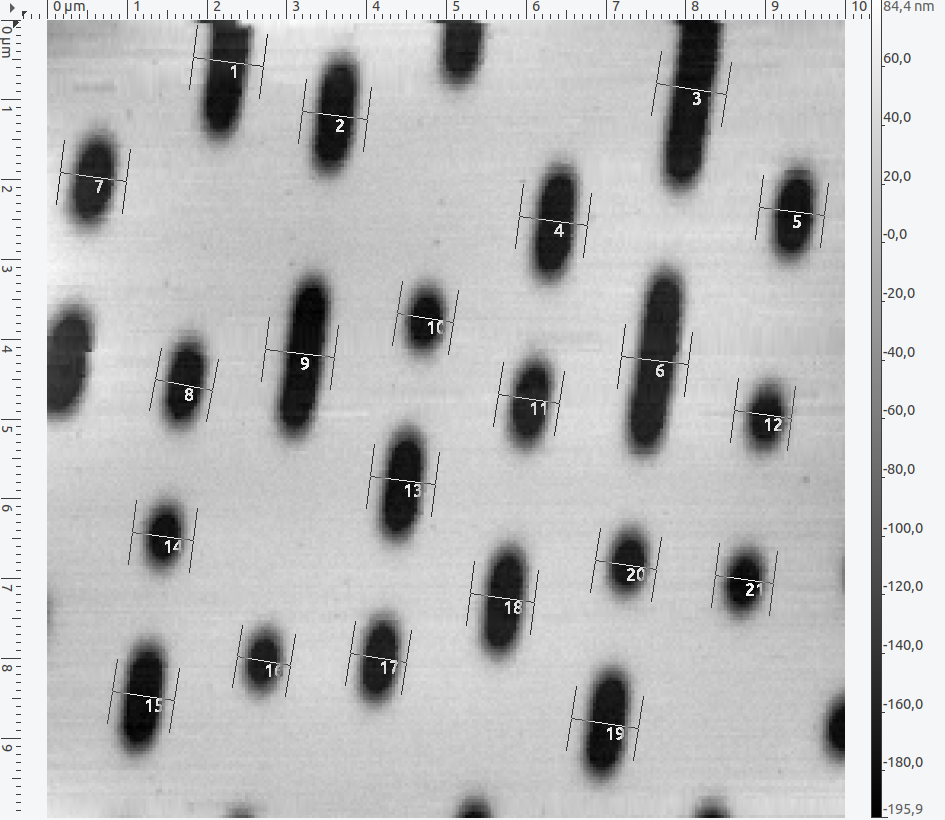
\includegraphics[width=\textwidth]{AFM_auswertung/cd_tiefe.png}
	\caption{.}
	\label{abb:}
	\end{subfigure}
	~
	\begin{subfigure}[t]{0.3\textwidth}
	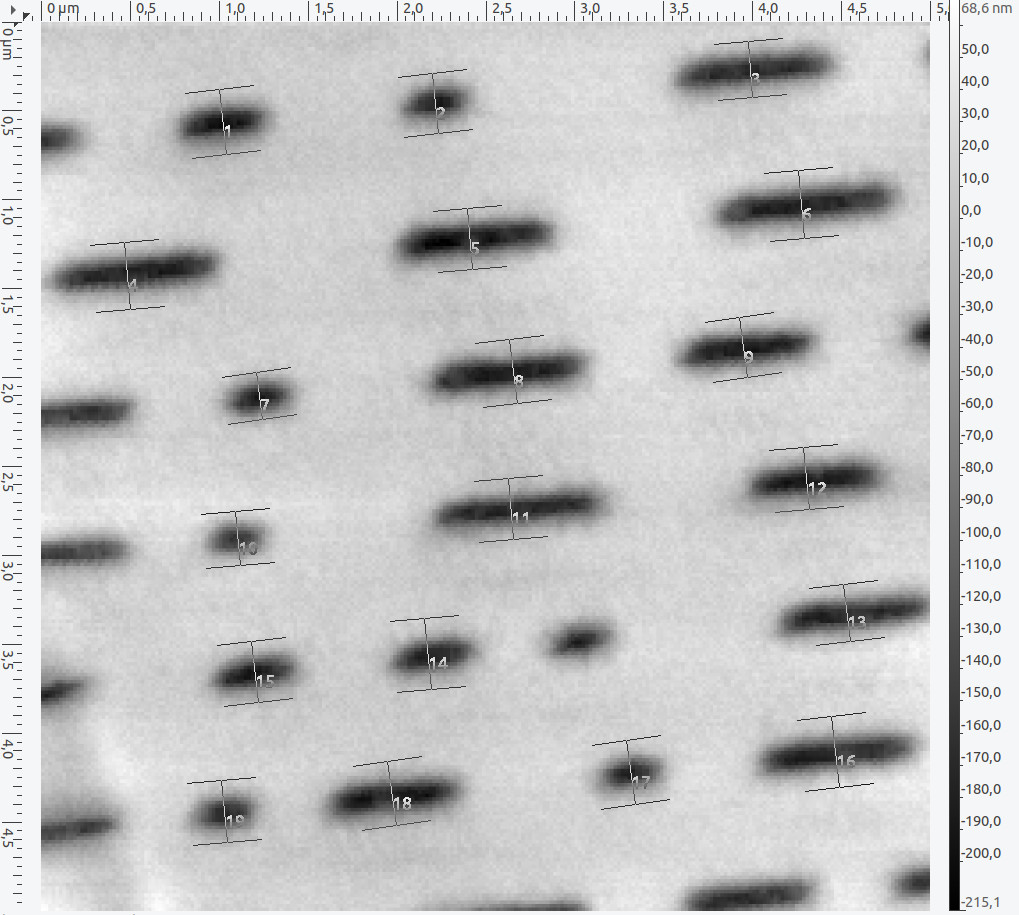
\includegraphics[width=\textwidth]{AFM_auswertung/dvd_tiefe.png}
	\caption{.}
	\label{abb:}
	\end{subfigure}
	~
	\begin{subfigure}[t]{0.3\textwidth}
	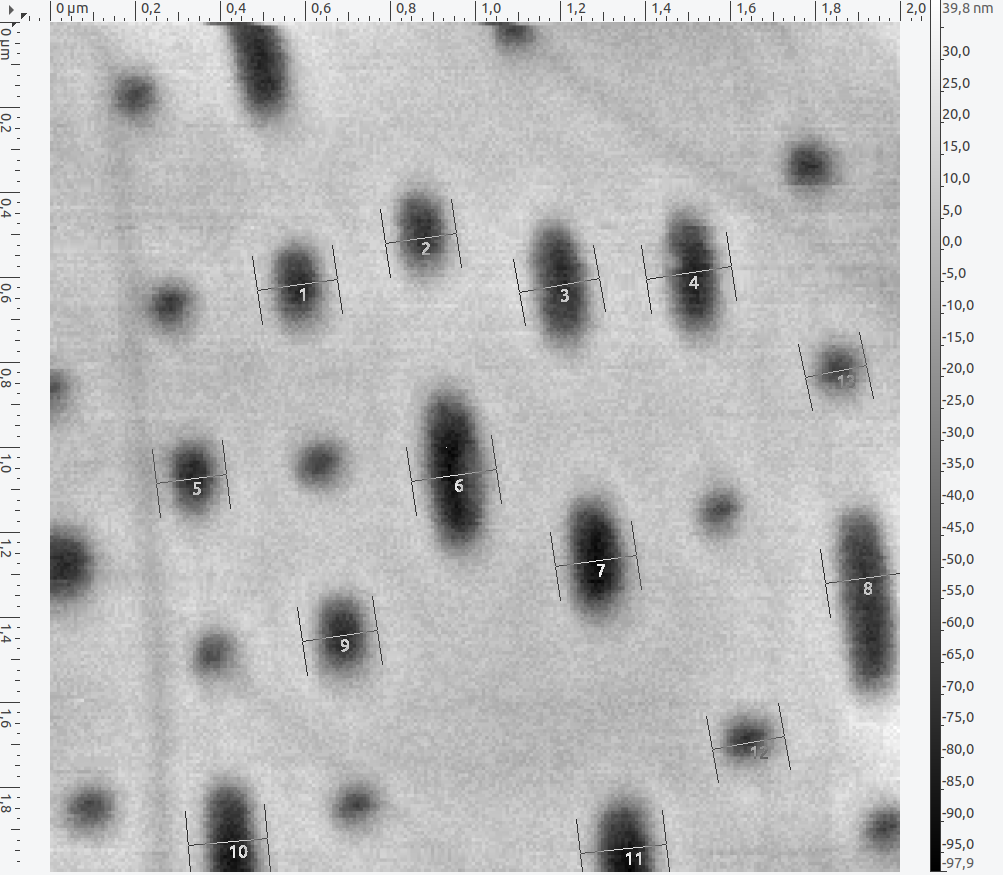
\includegraphics[width=\textwidth]{AFM_auswertung/bluray_tiefe.png}
	\caption{.}
	\label{abb:}
	\end{subfigure}
	\\
	\begin{subfigure}[t]{0.3\textwidth}
	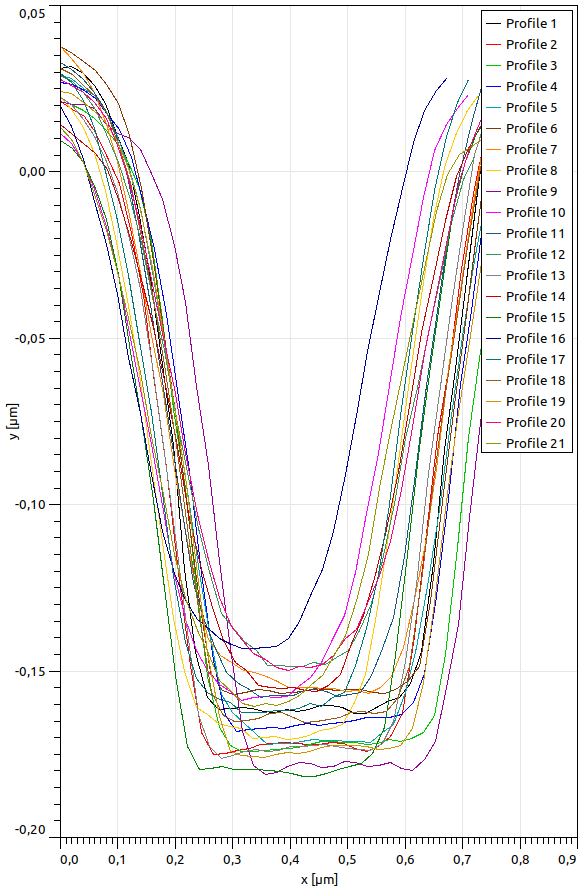
\includegraphics[width=\textwidth]{AFM_auswertung/cd_tiefe_grafik.png}
	\caption{.}
	\label{abb:}
	\end{subfigure}
	~
	\begin{subfigure}[t]{0.3\textwidth}
	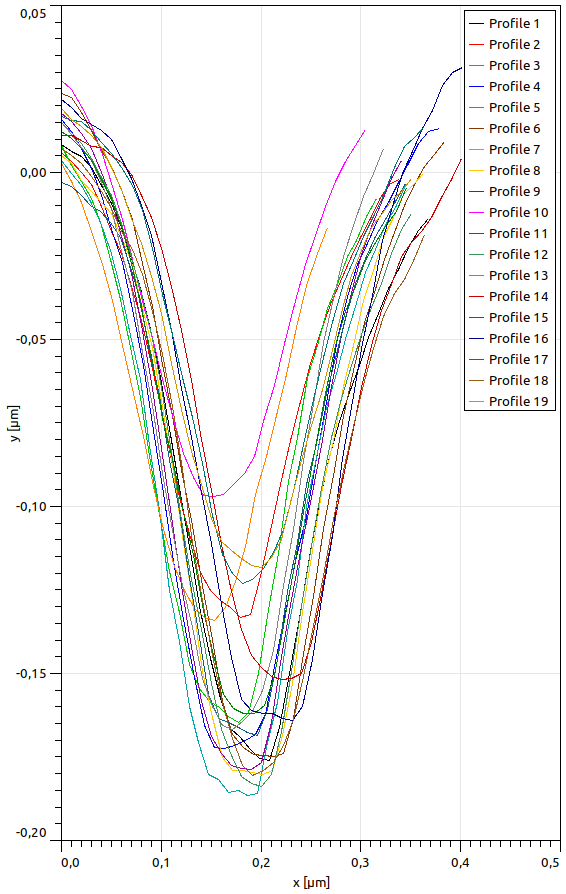
\includegraphics[width=\textwidth]{AFM_auswertung/dvd_tiefe_grafik.png}
	\caption{.}
	\label{abb:}
	\end{subfigure}
	~
	\begin{subfigure}[t]{0.3\textwidth}
	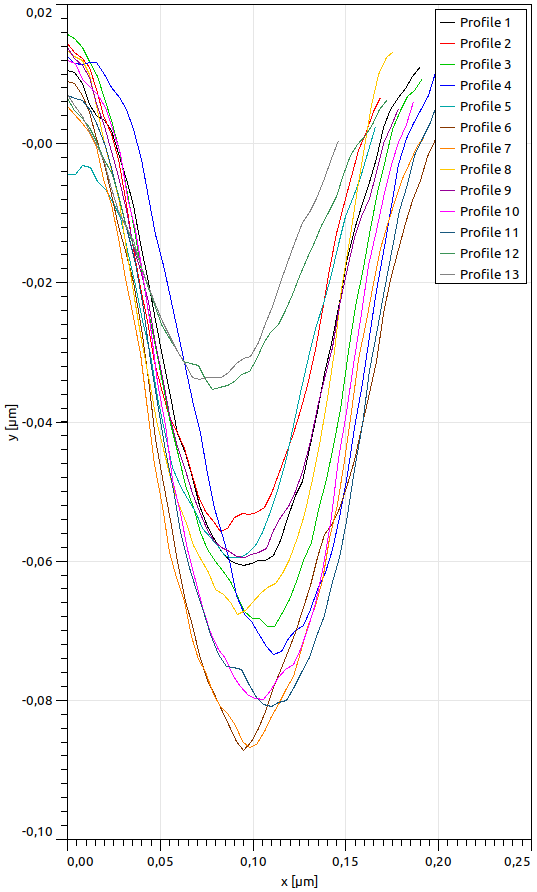
\includegraphics[width=\textwidth]{AFM_auswertung/bluray_tiefe_grafik.png}
	\caption{.}
	\label{abb:}
	\end{subfigure}
\caption{.}
\label{abb:pit_tiefe}
\end{figure}


\begin{table}
	\centering
	\caption{.}
\begin{tabular}{|r|ccc|}
	\hline
	{} & {CD} & {DVD} & {Blueray} \\
	\hline
	Pitabstand / $\mu m$ & $1,459 \pm 0,031$ & $0,778 \pm 0,014$ & $0,314 \pm 0,008$ \\
	Pitbreite	/ $\mu m$ &	$0,454 \pm 0,023$ & $0,153 \pm 0,009$ & $0,102 \pm 0,008$ \\
	Minimale Pitlänge / $\mu m$ & $0,656 \pm 0,025$ & $0,299 \pm 0,022$ & $0,098 \pm 0,007$ \\
	Maximale Pitlänge / $\mu m$ & 2,127 & $0,858 \pm 0,022$ & 0,436 \\
	Pittiefe /  &  &  &  \\
	\hline
\end{tabular}
\label{tab:auf2}
\end{table}


\subsection{Federkonstante, Adhäsionskraft, Elastizitätsmodul mittels Kraft-Abstandskurven}

\begin{figure}[H]
\centering
	\begin{subfigure}[t]{0.3\textwidth}
	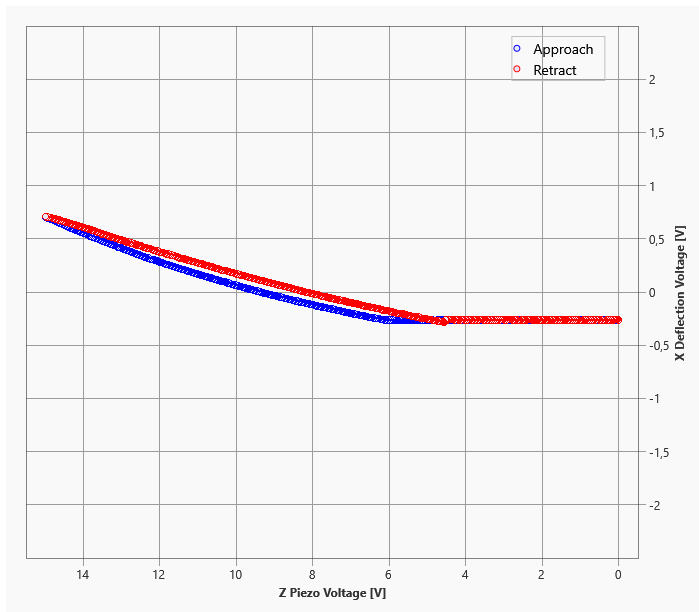
\includegraphics[width=\textwidth]{AFM_auswertung/edelstahl_kurve.png}
	\caption{.}
	\label{abb:}
	\end{subfigure}
	\\
	\begin{subfigure}[t]{0.3\textwidth}
	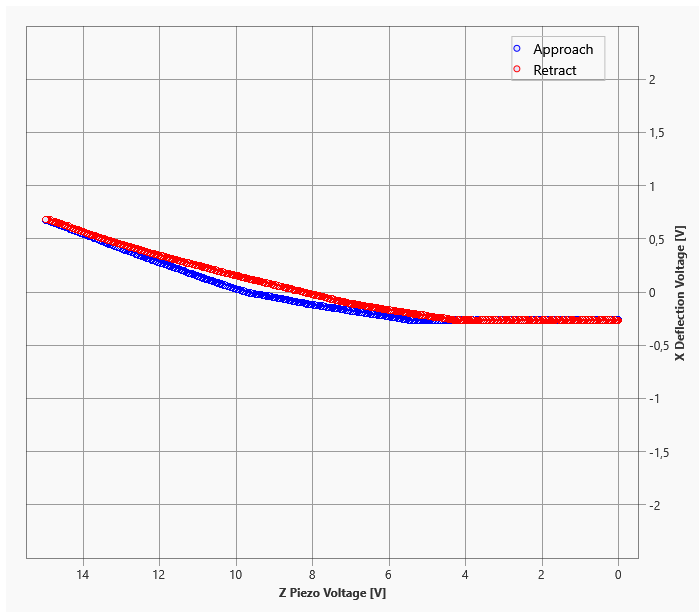
\includegraphics[width=\textwidth]{AFM_auswertung/teflon_kurve.png}
	\caption{.}
	\label{abb:}
	\end{subfigure}
	\\
	\begin{subfigure}[t]{0.3\textwidth}
	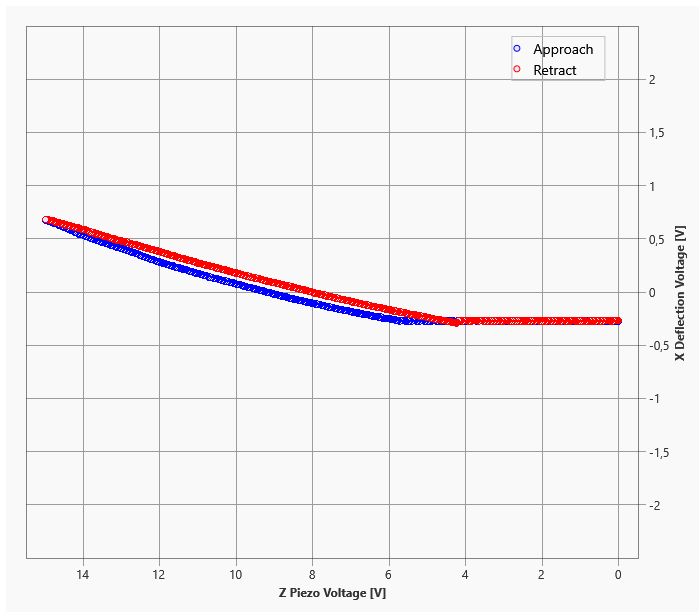
\includegraphics[width=\textwidth]{AFM_auswertung/TiN_kurve.png}
	\caption{.}
	\label{abb:}
	\end{subfigure}
\caption{.}
\label{abb:auf3}
\end{figure}

